\section{A recurring loop must survive its own operating history}

\subsection{One start, durable boundaries and selective stopping}

The research launcher explicitly starts one finite campaign. Within each stream the released workbench adapter produces the result pack while the research controller advances Identify, discovery, construction, qualification, admission and the next permitted mission. It persists accepted results, rejected candidates, charged work and source-bound methods. The end of useful authorized work is a WAIT/COMPLETE outcome, not an instruction to manufacture more demand.

A separate-process fault campaign executed 12 checks before confirmation. Its source identity is preserved as \artifact{e395004b}; the final \artifact{7e5a1dd2} bundle adds native fallback reporting, and the review records that exact delta instead of relabelling earlier tests. The exercised operating mechanisms and separate checker remain unchanged. All 12 checks pass in that campaign, with raw failed-process exit codes, checkpoints, guards and result receipts retained.

\begin{table}[ht]\centering\small
\begin{tabularx}{\linewidth}{L{39mm}Y}
\toprule
Operating condition & Executed observation \\
\midrule
Restart / lost acknowledgement & A process exits after durable acceptance; restart completes three missions with three mission executions. Repeating the completed request adds no execution. \\
Interrupted intent & An unacknowledged attempt charges its full 94,284-unit reservation before recovery. Exactly-once CPU execution is not claimed. \\
STOP and resume & The first accepted receipt remains byte-identified; explicit resume completes the finite stream. \\
Changed dependency or source & The old snapshot is refused against the current configuration/source identity. \\
Invalid receipt & A changed schedule with recomputed outer hashes still fails the separate current checker. \\
Budget, expiry and wall deadline & Exhausted work, expired or malformed authority and a finite wall boundary stop further work. No retry renews the limit. \\
Stale state / rejected descendant & An older same-cursor paid checkpoint is refused; rollback restores the portfolio; retry or rehashed restore cannot resurrect the rejected asset. \\
Unresponsive checker & The subprocess times out, delivers no accepted result and charges the 3,620-unit checker reservation. \\
\bottomrule
\end{tabularx}
\caption{Twelve source-bound development checks grouped by failure boundary. Raw evidence is under \artifact{development/operating-faults-final/}; the exact-source review is \artifact{review/MAIN_PRE_FREEZE_REVIEW.json}.}
\end{table}

A durable intent reserves the next execution. A ready result permits recovery without recomputing an already accepted effect. A monotone guard retains expenditure, sequence and rejection history so that a well-formed but stale snapshot cannot refund paid discovery. Recovery still performs a new check: integrity and freshness do not establish correctness by themselves. The local guard and hashes do not defend against an administrator who can rewrite the entire host and all evidence.

\begin{figure}[ht]\centering
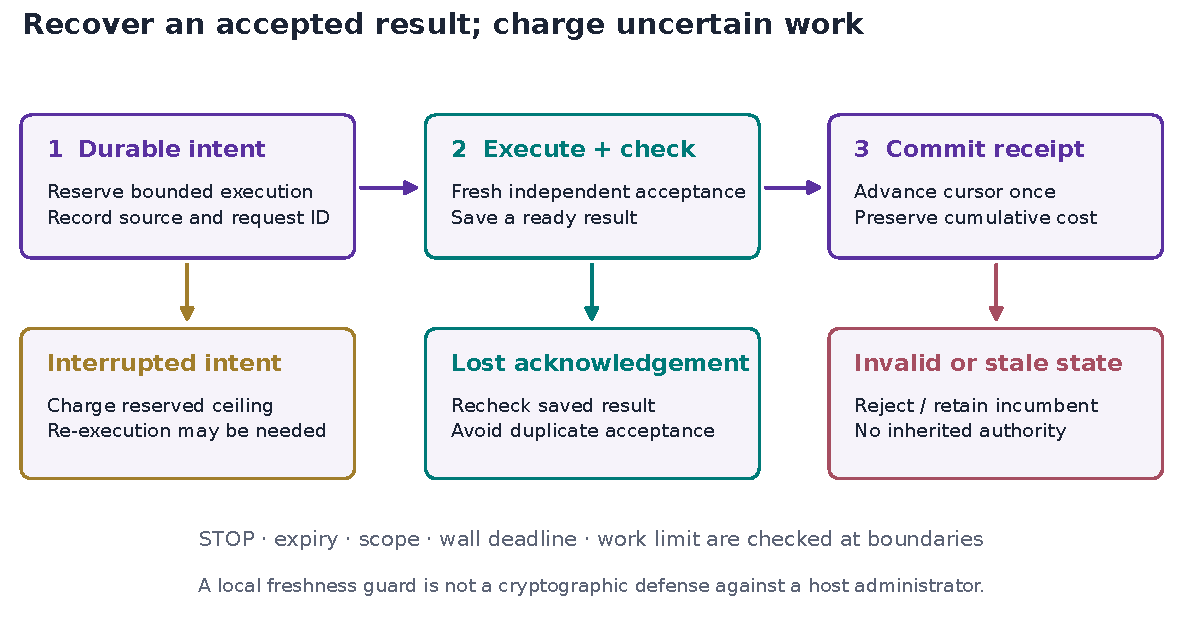
\includegraphics[width=\linewidth]{figures/failure-recovery-map.pdf}
\caption{Failure and recovery boundaries. Accepted-result deduplication and conservative charging of uncertain work are different guarantees.}
\end{figure}

\subsection{Storage, maintenance and bounded load}

The controller limits the active catalogue to three source-bound assets. Lookup, retrieval, current checking, admission and checkpoint growth are paid by the declared tariff. Replaced, stale or rolled-back assets lose applicability; their evidence remains in the research archive. Keeping historical failures is useful for audit but is not a zero-cost production retention policy. The finite experiment reports physical stored bytes and charges serialization blocks. It does not establish indefinite archival economics or a storage-leak-free long-running service.

The registered load probe completes 85/85 valid schedules, of which 68 meet their deadlines, in batches of 1, 4, 16 and 64 with at most four concurrent checker processes. Observed throughput rises from 21.06 to 37.07, 51.09 and 56.95 tasks per second; the 95th-percentile enqueue-to-durable latency rises from 37.63 to 89.63, 288.45 and 1,018.46\,ms. No batch exhausts its deadline, and no mid-batch manual intervention occurs. These are finite local measurements, including queueing, input preparation, evidence writes and checker startup/shutdown. They do not establish sustained throughput under arbitrary load.

The complete confirmatory campaign uses one explicit launch for 336 stream/treatment executions and 72 native reference calls, with zero manually triggered intermediate phases. It takes 844.40 seconds of elapsed time and 751.10 seconds of measured Node CPU; the separate Python CPU total is unavailable. Common synthetic WORLD construction takes 420.61\,ms and includes 3,464,226 known baseline-generation units, reported separately from conditional per-arm mission work. Setup, authoring, review and the additional historical replay remain research effort, not free autonomous output.

The 336 completed trial directories occupy 209,075,637 bytes in total, with final checkpoints ranging from 89,913 to 442,729 bytes. In the primary flywheel arm, checkpoint serialization alone costs 5,238,180 of 11,714,786 charged units (44.71\%). Retention cannot be evaluated as though its history were free. These full research snapshots are not an optimal archival design; an incrementally stored journal could change this cost boundary and would require its own measured comparison.


\begin{figure}[ht]\centering
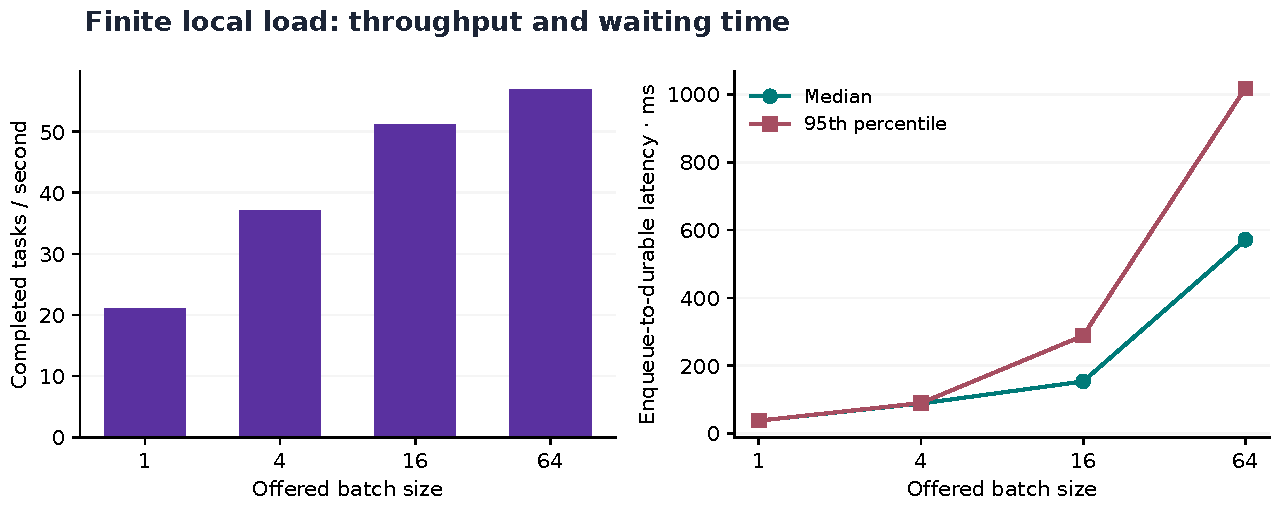
\includegraphics[width=\linewidth]{figures/finite-load.pdf}
\caption{One local observation per batch, at most four in flight. Latency includes queueing through durable evidence write. Task mixtures differ slightly across the small batches, and the host is not a dedicated production environment. These measurements do not establish a service-level objective or general scalability.}
\end{figure}

\subsection{The browser is an instrument, not an animation}

The standalone browser opens with a nine-job synthetic release, three available workers and a 28-hour target. Its fresh computation yields a valid 23-hour plan; all nine jobs pass the separate browser checker. Global optimality is not claimed. The user can edit jobs, dependencies, durations, crew and calendar, inspect the schedule as a table or chart, and download JSON/CSV evidence. No account, installation, wallet, API key or network connection is required.

A second action starts the six-mission bounded stream. The interface shows the current result, exact retained strategy, candidate/incumbent checks, full browser charges and the next requirement. A separate construction-laboratory action labels correctness-only retention. The research-results panel is explicitly recorded evidence; opening it does not rerun confirmation. Browser checker units and the main Python-backed reference counts are distinct measurements.

One development recovery failure is preserved rather than erased: reopening identical HTML regenerated a fixture-accounting value from 6,096 to 6,115, which correctly triggered a configuration mismatch. The scientific interpreter now uses explicitly metered deterministic insertion sorting; browser fixtures have fixed source bytes and construction provenance. Final frozen-source browser checks cover 18 checker assertions, 11 useful-plan/authority/layout checks, eight stream/recovery checks and five recorded-table checks. The exact HTML hashes and the failed original state are retained.

Closing the tab stops browser computation. Saved history supports an explicit later resume. The local Node companion can continue while its explicitly started process remains running; no hosted agent, native installed operator or unattended production service is represented by the page.
